%==============================================================================
%  ECG Holter Monitor -- Technical / Developer Manual
%  Master document. Compile with:  latexmk -pdf main.tex
%  (or: pdflatex main.tex  x2,  then  bibtex main,  then pdflatex x2)
%==============================================================================
\documentclass[11pt,a4paper]{article}

%------------------------------------------------------------------ packages
\usepackage[utf8]{inputenc}
\usepackage[T1]{fontenc}
\usepackage{lmodern}
\usepackage[a4paper,margin=2.5cm]{geometry}
\usepackage{graphicx}
\usepackage{xcolor}
\usepackage{amsmath}
\usepackage{booktabs}
\usepackage{caption}
\usepackage{listings}
\usepackage{fancyhdr}
\usepackage{enumitem}
\usepackage{tikz}
\usetikzlibrary{arrows.meta,positioning,shapes.geometric,calc,fit,backgrounds}
\usepackage[hidelinks]{hyperref}

%------------------------------------------------------------------ colours
\definecolor{accent}{RGB}{0,110,90}
\definecolor{accentlight}{RGB}{224,242,238}
\definecolor{hwcol}{RGB}{210,235,255}
\definecolor{bkcol}{RGB}{255,236,214}
\definecolor{fecol}{RGB}{226,222,247}
\definecolor{codebg}{RGB}{248,248,248}
\definecolor{codecomment}{RGB}{110,120,120}
\definecolor{codekw}{RGB}{0,90,160}
\definecolor{codestr}{RGB}{160,60,30}
\definecolor{linenum}{RGB}{160,160,160}

%------------------------------------------------------------------ listings
\lstdefinestyle{base}{
  backgroundcolor=\color{codebg},
  basicstyle=\ttfamily\footnotesize,
  keywordstyle=\color{codekw}\bfseries,
  commentstyle=\color{codecomment}\itshape,
  stringstyle=\color{codestr},
  numberstyle=\tiny\color{linenum},
  numbers=left,
  numbersep=8pt,
  frame=single,
  rulecolor=\color{linenum!60},
  framesep=6pt,
  breaklines=true,
  showstringspaces=false,
  tabsize=2,
  columns=fullflexible,
  keepspaces=true,
  captionpos=b,
}
\lstdefinestyle{cpp}{style=base,language=C++}
\lstdefinestyle{py}{style=base,language=Python}
\lstdefinestyle{js}{style=base,language=Java}   % JS not built-in; Java highlighting is close
\lstdefinestyle{jsonsty}{style=base}

%------------------------------------------------------------------ headers
\pagestyle{fancy}
\fancyhf{}
\setlength{\headheight}{14pt}
\lhead{\small\textsc{ECG Holter Monitor}}
\rhead{\small Technical Manual}
\cfoot{\thepage}
\renewcommand{\headrulewidth}{0.4pt}

\captionsetup{font=small,labelfont=bf}

%------------------------------------------------------------------ tikz styles
\tikzset{
  block/.style   ={rectangle, rounded corners=3pt, draw=black!55, thick,
                   align=center, minimum height=11mm, minimum width=26mm, font=\small},
  hw/.style      ={block, fill=hwcol},
  bk/.style      ={block, fill=bkcol},
  fe/.style      ={block, fill=fecol},
  stage/.style   ={rectangle, rounded corners=2pt, draw=accent, thick,
                   fill=accentlight, align=center, text width=82mm,
                   minimum height=9mm, font=\small},
  flow/.style    ={-{Stealth[length=3mm]}, thick},
  lbl/.style     ={font=\scriptsize\itshape, fill=white, inner sep=1pt},
}

%==============================================================================
\begin{document}

%------------------------------------------------------------------ title page
\begin{titlepage}
  \centering
  \vspace*{2.5cm}
  {\Huge\bfseries Wearable ECG Holter Monitor\par}
  \vspace{0.6cm}
  {\Large with an ESP32 Acquisition Node and a Remote Real-Time Dashboard\par}
  \vspace{1.4cm}
  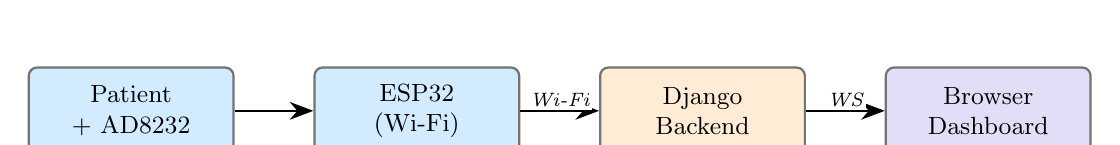
\begin{tikzpicture}
    \node[hw] (a) {Patient\\ + AD8232};
    \node[hw, right=10mm of a] (b) {ESP32\\ (Wi-Fi)};
    \node[bk, right=10mm of b] (c) {Django\\ Backend};
    \node[fe, right=10mm of c] (d) {Browser\\ Dashboard};
    \draw[flow] (a) -- (b);
    \draw[flow] (b) -- (c) node[midway,above,lbl]{Wi-Fi};
    \draw[flow] (c) -- (d) node[midway,above,lbl]{WS};
  \end{tikzpicture}
  \vspace{1.6cm}

  {\large\textbf{Technical \& Developer Manual}\par}
  \vspace{2.0cm}
  {\large Salwan Aldhahab\par}
  \vspace{0.4cm}
  {\large\today\par}
  \vfill
  {\small This document describes the design, data flow, signal processing and
  operation of the ECG Holter Monitor project.\par}
\end{titlepage}

%------------------------------------------------------------------ toc
\tableofcontents
\thispagestyle{fancy}
\clearpage

%------------------------------------------------------------------ abstract
\section*{About this document}
\addcontentsline{toc}{section}{About this document}
This is a developer-oriented manual for the \emph{ECG Holter Monitor}, a wearable
single-lead electrocardiogram (ECG) acquisition device that streams a patient's
heart waveform to a remote dashboard in real time. The system has three
cooperating parts: an ESP32 microcontroller node that digitises the analog ECG
signal, a Django/Channels backend that cleans the signal with a digital signal
processing (DSP) pipeline, and a browser dashboard that renders the live waveform.
Each part is documented in its own section, followed by an end-to-end data-flow
description, build/run instructions, and a list of known limitations.
\clearpage

%------------------------------------------------------------------ sections
%==============================================================================
\section{System Overview}
%==============================================================================

\subsection{What the system does}
A Holter monitor is a portable device that records a patient's ECG continuously
while they go about normal activity. This project implements a modern, networked
variant: instead of storing the signal on the device for later review, the
wearable node \emph{streams} the heart waveform over Wi-Fi so that a clinician
can watch it live on a remote dashboard from anywhere on the network.

The patient wears a small enclosure containing an ESP32 microcontroller and an
\textbf{AD8232} single-lead ECG analog front-end. Three electrodes on the body
feed the heart's electrical activity into the AD8232, which conditions it into a
clean analog voltage. The ESP32 samples that voltage with its on-chip
analog-to-digital converter (ADC) and pushes batches of samples to a server. The
server filters the raw signal and broadcasts the result to every connected
browser, where it is drawn as a scrolling waveform.

\subsection{High-level architecture}
The system is split into three tiers, summarised in
Figure~\ref{fig:architecture}.

\begin{description}[leftmargin=2.2cm,style=nextline]
  \item[Acquisition] The ESP32 + AD8232 wearable node. Reads the analog ECG on
        \texttt{GPIO36} at $\approx$\,250\,Hz and transmits 250-sample JSON
        batches (one batch $\approx$ one second) over a Wi-Fi WebSocket.
  \item[Processing] A Django backend running on the Channels/Daphne ASGI stack.
        A WebSocket consumer receives each batch, runs an eight-stage DSP filter,
        and fans the cleaned signal out to all dashboard clients.
  \item[Visualisation] A single-page browser dashboard using Chart.js. It keeps a
        rolling 1000-sample buffer and redraws the live trace as data arrives.
\end{description}

\begin{figure}[h]
  \centering
  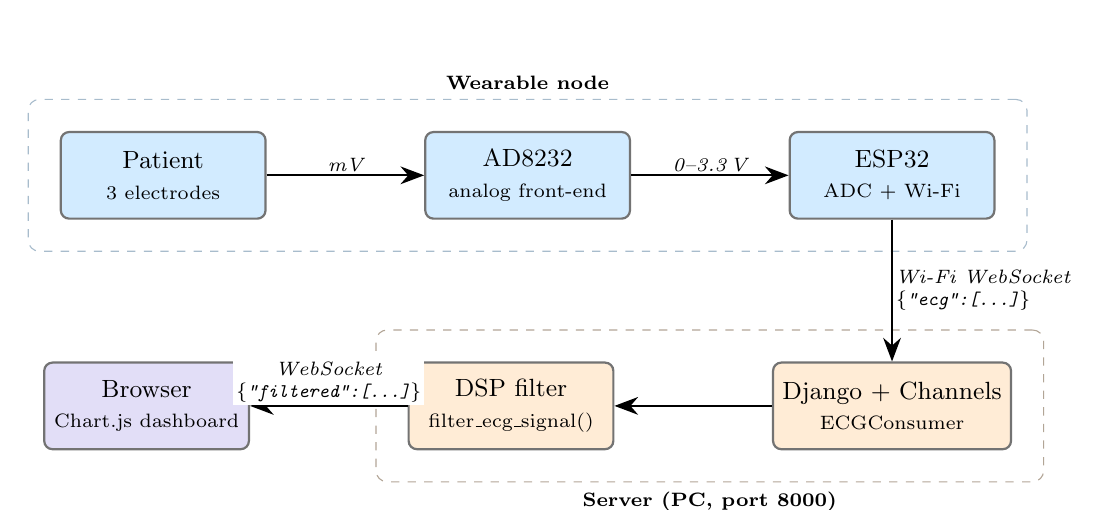
\begin{tikzpicture}[node distance=16mm and 20mm]
    % nodes
    \node[hw] (pat) {Patient\\\scriptsize 3 electrodes};
    \node[hw, right=of pat] (afe) {AD8232\\\scriptsize analog front-end};
    \node[hw, right=of afe] (esp) {ESP32\\\scriptsize ADC + Wi-Fi};
    \node[bk, below=18mm of esp] (srv) {Django + Channels\\\scriptsize ECGConsumer};
    \node[bk, left=of srv] (dsp) {DSP filter\\\scriptsize filter\_ecg\_signal()};
    \node[fe, left=of dsp] (web) {Browser\\\scriptsize Chart.js dashboard};

    % flows
    \draw[flow] (pat) -- (afe) node[midway,above,lbl]{mV};
    \draw[flow] (afe) -- (esp) node[midway,above,lbl]{0--3.3\,V};
    \draw[flow] (esp) -- (srv)
       node[midway,right,lbl,align=left]{Wi-Fi WebSocket\\\texttt{\{"ecg":[...]\}}};
    \draw[flow] (srv) -- (dsp);
    \draw[flow] (dsp) -- (web)
       node[midway,above,lbl,align=center]{WebSocket\\\texttt{\{"filtered":[...]\}}};

    % grouping backgrounds
    \begin{scope}[on background layer]
      \node[draw=hwcol!80!black, dashed, rounded corners, fit=(pat)(afe)(esp),
            inner sep=4mm, label={[font=\scriptsize\bfseries]above:Wearable node}] {};
      \node[draw=bkcol!70!black, dashed, rounded corners, fit=(dsp)(srv),
            inner sep=4mm, label={[font=\scriptsize\bfseries]below:Server (PC, port 8000)}] {};
    \end{scope}
  \end{tikzpicture}
  \caption{End-to-end architecture. The wearable node digitises and transmits raw
  ECG; the server filters it and broadcasts the cleaned waveform to the dashboard.}
  \label{fig:architecture}
\end{figure}

\subsection{Technology stack}
\begin{table}[h]
  \centering
  \small
  \begin{tabular}{@{}lll@{}}
    \toprule
    \textbf{Tier} & \textbf{Technology} & \textbf{Role} \\
    \midrule
    Acquisition  & ESP32 (Arduino C++)        & Sampling and Wi-Fi transport \\
                 & AD8232                     & Single-lead ECG analog front-end \\
                 & ArduinoWebsockets, ArduinoJson & WebSocket client + JSON encoding \\
    Processing   & Python 3, Django 5.1.7     & Web application framework \\
                 & Django Channels + Daphne   & ASGI / WebSocket handling \\
                 & NumPy, SciPy, PyWavelets   & ECG signal-processing pipeline \\
    Visualisation& HTML5 + JavaScript         & Single-page dashboard \\
                 & Chart.js 4.4.1             & Real-time line chart \\
    \bottomrule
  \end{tabular}
  \caption{Components used at each tier of the system.}
  \label{tab:stack}
\end{table}

\subsection{Repository layout}
The relevant source lives in two top-level folders:
\begin{lstlisting}[style=base,numbers=none]
HolterMonitor/
|-- arduino/
|   `-- websocket_ecg_send_data/
|       `-- websocket_ecg_send_data.ino   <- ESP32 firmware
`-- holter_monitor/                       <- Django project
    |-- manage.py
    |-- send_fake_data.py                 <- hardware-free ECG simulator
    |-- holter_monitor/                   <- project package
    |   |-- settings.py  asgi.py  urls.py
    `-- ecg/                              <- the ECG app
        |-- consumers.py   <- WebSocket consumer (ECGConsumer)
        |-- routing.py     <- ws/ecg/ route
        |-- filters.py     <- 8-stage DSP pipeline
        |-- views.py       <- serves the dashboard page
        `-- templates/ecg.html            <- Chart.js dashboard
\end{lstlisting}

%==============================================================================
\section{Hardware \& Firmware}
%==============================================================================

\subsection{Signal chain}
The heart's electrical activity reaches the digital domain through the chain shown
in Figure~\ref{fig:wiring}. Three electrodes (right arm, left arm, right leg
reference) connect to the \textbf{AD8232}, a single-lead, integrated ECG analog
front-end. The AD8232 performs instrumentation amplification, a built-in
right-leg-drive to reject common-mode interference, and band-pass filtering,
producing a single-ended output centred in the ESP32's input range. That output
drives \texttt{GPIO36} (ADC1 channel 0, the input-only ``VP'' pin), which the
ESP32 samples with its 12-bit ADC, yielding integer codes in the range
$0$--$4095$.

\begin{figure}[h]
  \centering
  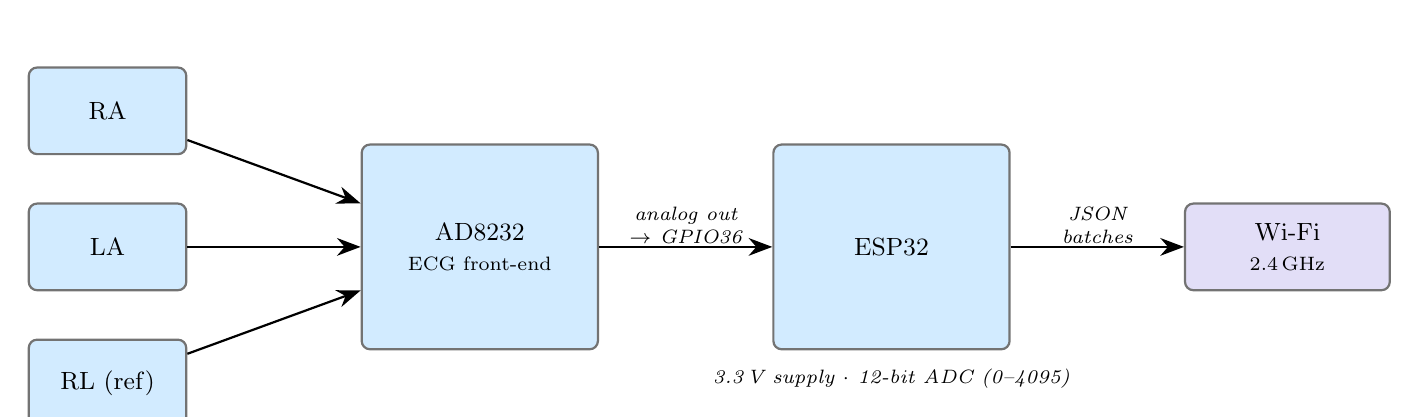
\begin{tikzpicture}[node distance=14mm and 22mm]
    \node[hw, minimum width=20mm] (ra)  {RA};
    \node[hw, minimum width=20mm, below=6mm of ra] (la) {LA};
    \node[hw, minimum width=20mm, below=6mm of la] (rl) {RL (ref)};
    \node[hw, right=of la, minimum width=30mm, minimum height=26mm] (afe) {AD8232\\\scriptsize ECG front-end};
    \node[hw, right=of afe, minimum width=30mm, minimum height=26mm] (esp) {ESP32};
    \node[fe, right=of esp, minimum width=26mm] (net) {Wi-Fi\\\scriptsize 2.4\,GHz};

    \draw[flow] (ra) -- (afe);
    \draw[flow] (la) -- (afe);
    \draw[flow] (rl) -- (afe);
    \draw[flow] (afe) -- (esp)
        node[midway,above,lbl,align=center]{analog out\\$\rightarrow$ GPIO36};
    \draw[flow] (esp) -- (net)
        node[midway,above,lbl,align=center]{JSON\\batches};

    \node[lbl, below=2mm of esp, align=center]
        {3.3\,V supply $\cdot$ 12-bit ADC (0--4095)};
  \end{tikzpicture}
  \caption{Hardware signal chain: electrodes $\rightarrow$ AD8232 $\rightarrow$
  ESP32 ADC on GPIO36 $\rightarrow$ Wi-Fi.}
  \label{fig:wiring}
\end{figure}

\begin{table}[h]
  \centering
  \small
  \begin{tabular}{@{}ll@{}}
    \toprule
    \textbf{Parameter} & \textbf{Value} \\
    \midrule
    Microcontroller        & ESP32 (Wi-Fi 2.4\,GHz) \\
    Analog front-end       & AD8232 single-lead ECG \\
    ADC input pin          & GPIO36 (ADC1\_CH0, input only) \\
    ADC resolution         & 12-bit, codes 0--4095 \\
    Sampling rate          & $\approx$250\,Hz (\texttt{SAMPLE\_DELAY\_MS = 4}) \\
    Batch size             & 250 samples (\texttt{SAMPLE\_COUNT}) \\
    Batch period           & $\approx$1\,s per transmission \\
    Transport              & WebSocket over Wi-Fi, server port 8000 \\
    Endpoint               & \texttt{ws://<server>:8000/ws/ecg/} \\
    \bottomrule
  \end{tabular}
  \caption{Key acquisition parameters, taken from the firmware.}
  \label{tab:hwparams}
\end{table}

\subsection{Wiring schematic}
At the connector level the build is deliberately minimal: the firmware only ever
calls \texttt{analogRead(36)}, so just three wires are required between the AD8232
module and the ESP32 --- power, ground and the analog output.
Figure~\ref{fig:schematic} shows the connections. The AD8232's lead-off detection
and shutdown pins (\texttt{LO+}, \texttt{LO-}, \texttt{SDN}) are left unconnected
because the firmware does not read them; they are optional inputs for detecting a
detached electrode.

\begin{figure}[h]
  \centering
  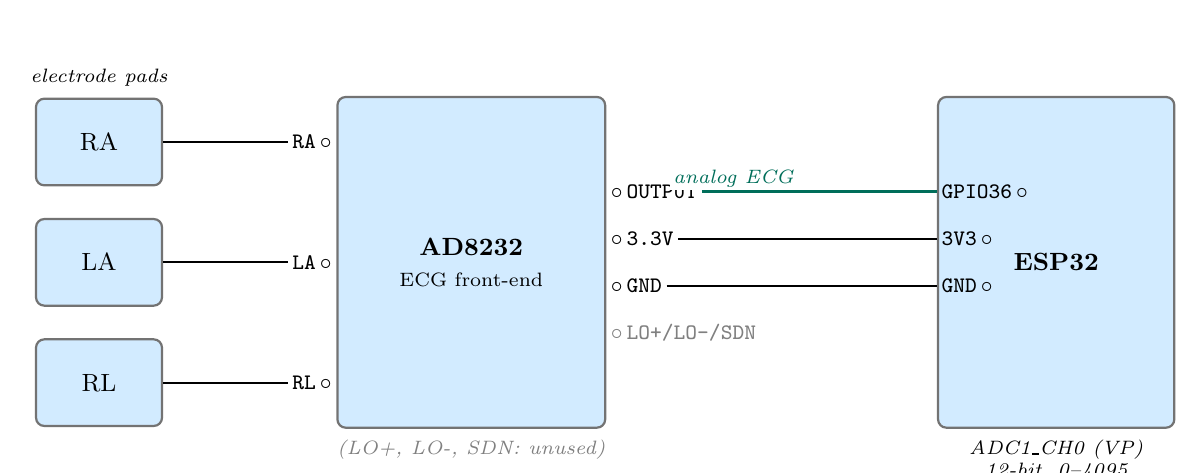
\begin{tikzpicture}[font=\small,
      pin/.style={font=\footnotesize\ttfamily, inner sep=1.5pt},
      wire/.style={thick}]
    % electrodes (left)
    \node[hw, minimum width=16mm] (era) {RA};
    \node[hw, minimum width=16mm, below=4mm of era] (ela) {LA};
    \node[hw, minimum width=16mm, below=4mm of ela] (erl) {RL};
    \node[lbl, above=1mm of era] {electrode pads};

    % AD8232 module (middle) with explicit pin anchors
    \node[hw, right=22mm of ela, minimum width=34mm, minimum height=42mm,
          align=center] (afe) {\textbf{AD8232}\\\scriptsize ECG front-end};
    % left-side pins (electrode inputs)
    \node[pin, anchor=east] (p_ra) at (afe.west |- era) {RA\,$\circ$};
    \node[pin, anchor=east] (p_la) at (afe.west |- ela) {LA\,$\circ$};
    \node[pin, anchor=east] (p_rl) at (afe.west |- erl) {RL\,$\circ$};
    % right-side pins
    \node[pin, anchor=west] (p_out) at ($(afe.east)+(0,0.9)$)  {$\circ$\,OUTPUT};
    \node[pin, anchor=west] (p_33)  at ($(afe.east)+(0,0.3)$)  {$\circ$\,3.3V};
    \node[pin, anchor=west] (p_gnd) at ($(afe.east)+(0,-0.3)$) {$\circ$\,GND};
    \node[pin, anchor=west, text=gray] (p_lo)  at ($(afe.east)+(0,-0.9)$)
        {$\circ$\,LO+/LO-/SDN};
    \node[lbl, text=gray, below=1mm of afe] {(LO+, LO-, SDN: unused)};

    % ESP32 (right) with explicit pin anchors
    \node[hw, right=42mm of afe, minimum width=30mm, minimum height=42mm,
          align=center] (esp) {\textbf{ESP32}};
    \node[pin, anchor=west] (e_36)  at ($(esp.west)+(0,0.9)$)  {GPIO36\,$\circ$};
    \node[pin, anchor=west] (e_33)  at ($(esp.west)+(0,0.3)$)  {3V3\,$\circ$};
    \node[pin, anchor=west] (e_gnd) at ($(esp.west)+(0,-0.3)$) {GND\,$\circ$};
    \node[lbl, below=1mm of esp, align=center] {ADC1\_CH0 (VP)\\12-bit, 0--4095};

    % electrode wires
    \draw[wire] (era.east) -- (p_ra.west);
    \draw[wire] (ela.east) -- (p_la.west);
    \draw[wire] (erl.east) -- (p_rl.west);

    % AD8232 -> ESP32 (the three real connections)
    \draw[wire, accent] (p_out.east) -- ++(0.4,0) |- (e_36.west)
        node[pos=0.25,above,lbl]{analog ECG};
    \draw[wire] (p_33.east)  -- ++(0.9,0) |- (e_33.west);
    \draw[wire] (p_gnd.east) -- ++(0.6,0) |- (e_gnd.west);
  \end{tikzpicture}
  \caption{Connector-level wiring. Three electrode pads feed the AD8232; only three
  wires reach the ESP32 --- \texttt{OUTPUT}$\rightarrow$\texttt{GPIO36},
  \texttt{3.3V}$\rightarrow$\texttt{3V3} and \texttt{GND}$\rightarrow$\texttt{GND}.
  The lead-off/shutdown pins are left unconnected.}
  \label{fig:schematic}
\end{figure}

\subsection{Firmware behaviour}
The firmware
(\texttt{arduino/websocket\_ecg\_send\_data/websocket\_ecg\_send\_data.ino})
runs three Arduino libraries: \texttt{WiFi.h} for connectivity,
\texttt{ArduinoWebsockets} for the WebSocket client, and \texttt{ArduinoJson} for
serialisation. On boot it joins the Wi-Fi network and opens a WebSocket to the
server. The main loop then repeatedly:

\begin{enumerate}[noitemsep]
  \item reads 250 ADC samples from \texttt{GPIO36}, pausing 4\,ms between samples
        (so each batch spans about one second of signal);
  \item packs the samples into a JSON object \texttt{\{"ecg":[\,\ldots\,]\}};
  \item sends the JSON over the WebSocket and polls the connection;
  \item if the socket has dropped, it transparently reconnects.
\end{enumerate}

The acquisition loop itself is shown below.

\begin{lstlisting}[style=cpp,caption={ESP32 sampling and transmit loop (abridged).}]
#define ECG_PIN 36
#define SAMPLE_COUNT 250
#define SAMPLE_DELAY_MS 4        // ~250 Hz sampling rate

void loop() {
  if (!client.available()) {     // auto-reconnect if dropped
    connectToWebSocket();
    delay(1000);
    return;
  }

  int ecg_values[SAMPLE_COUNT];
  for (int i = 0; i < SAMPLE_COUNT; i++) {
    ecg_values[i] = analogRead(ECG_PIN);   // 12-bit: 0..4095
    delay(SAMPLE_DELAY_MS);
  }

  StaticJsonDocument<4096> doc;
  JsonArray ecg_array = doc.createNestedArray("ecg");
  for (int i = 0; i < SAMPLE_COUNT; i++) ecg_array.add(ecg_values[i]);

  String json;
  serializeJson(doc, json);
  client.send(json);             // -> ws://<server>:8000/ws/ecg/
  client.poll();
}
\end{lstlisting}

\paragraph{Configuration.} The Wi-Fi credentials and the server's IP address are
compile-time constants near the top of the sketch. Before flashing, set them for
your environment:
\begin{lstlisting}[style=cpp,numbers=none]
const char* ssid                  = "<YOUR_WIFI_SSID>";
const char* password              = "<YOUR_WIFI_PASSWORD>";
const char* websocket_server_host = "<YOUR_PC_IP>";   // e.g. 192.168.1.20
const int   websocket_server_port = 8000;
\end{lstlisting}
\emph{Note:} the firmware in the repository hard-codes a real SSID, password and
IP. These are credentials and should be replaced with placeholders or moved to a
secrets header before sharing the code (see Section~\ref{sec:limitations}).

\subsection{Wearable enclosure}
The electronics are housed in a small enclosure worn against the torso, with the
three electrode leads routed to standard chest positions and the ESP32 and a
battery sitting in the body of the case. Figure~\ref{fig:case} gives a conceptual
view of the assembly and electrode placement.

\begin{figure}[h]
  \centering
  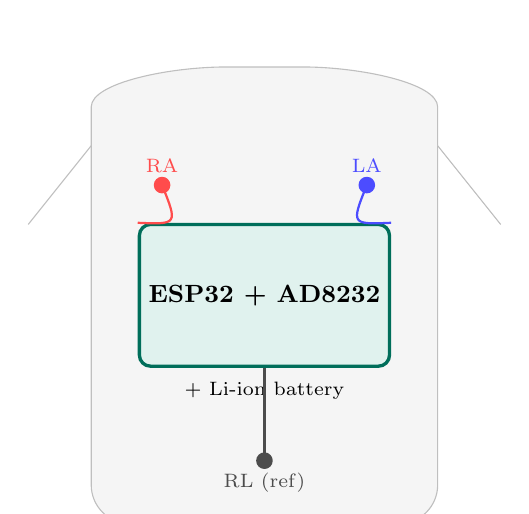
\begin{tikzpicture}[scale=1.0]
    % torso silhouette
    \draw[rounded corners=14pt, fill=gray!8, draw=gray!50]
        (-2.2,-3.2) -- (-2.2,1.6) .. controls (-2.2,2.4) and (-1.2,2.6) ..
        (0,2.6) .. controls (1.2,2.6) and (2.2,2.4) .. (2.2,1.6) --
        (2.2,-3.2) -- cycle;
    % shoulders
    \draw[gray!50, fill=gray!8] (-2.2,1.6) -- (-3.0,0.6);
    \draw[gray!50, fill=gray!8] (2.2,1.6) -- (3.0,0.6);

    % enclosure
    \node[draw=accent, very thick, fill=accentlight, rounded corners,
          minimum width=26mm, minimum height=18mm] (box) at (0,-0.3)
          {\small\bfseries ESP32 + AD8232};
    \node[font=\scriptsize, below=0.5mm of box] {+ Li-ion battery};

    % electrodes
    \fill[red!70]  (-1.3,1.1) circle (3pt) node[above=1pt,font=\scriptsize]{RA};
    \fill[blue!70] ( 1.3,1.1) circle (3pt) node[above=1pt,font=\scriptsize]{LA};
    \fill[black!70](-0.0,-2.4) circle (3pt) node[below=1pt,font=\scriptsize]{RL (ref)};

    % leads
    \draw[red!70, thick]  (-1.3,1.1) .. controls (-1.1,0.6) .. (box.north west);
    \draw[blue!70, thick] ( 1.3,1.1) .. controls ( 1.1,0.6) .. (box.north east);
    \draw[black!70, thick](-0.0,-2.4) -- (box.south);
  \end{tikzpicture}
  \caption{Conceptual view of the wearable enclosure and three-electrode
  placement. The case holds the ESP32, the AD8232 front-end and a battery.}
  \label{fig:case}
\end{figure}

\paragraph{Device photographs.} The figures below show the actual built hardware.
Each image is pulled from \texttt{doc/figures/}; if a file is ever absent, a framed
placeholder box is drawn in its place so the document always compiles (see
\texttt{figures/README.md}).

\newcommand{\photoslot}[3]{%
  % #1 = filename, #2 = caption, #3 = label
  \begin{figure}[h]\centering
    \IfFileExists{figures/#1}{%
      \includegraphics[width=0.7\linewidth]{figures/#1}%
    }{%
      \fbox{\begin{minipage}[c][32mm][c]{0.7\linewidth}\centering
        \ttfamily\small figures/#1\\[2pt]\normalfont\itshape (drop photo here)
      \end{minipage}}%
    }
    \caption{#2}\label{#3}
  \end{figure}}

\photoslot{device_assembled.jpg}{Assembled ESP32 + AD8232 unit inside its case.}{fig:photo-device}
\photoslot{electrodes.jpg}{The snap ECG electrodes used with the AD8232 front-end.}{fig:photo-electrodes}
\photoslot{case_worn.jpg}{The enclosure worn on the torso.}{fig:photo-worn}

%==============================================================================
\section{Backend: Django + Channels}
%==============================================================================

\subsection{Why ASGI and Channels}
A classic Django request/response cycle cannot hold a long-lived, bidirectional
connection open, which is exactly what streaming ECG needs. The project therefore
runs on the asynchronous \textbf{ASGI} stack: \textbf{Django Channels} adds
WebSocket support and \textbf{Daphne} serves the application. The same server
process handles ordinary HTTP (to serve the dashboard page) and WebSockets (to
carry ECG data).

The protocol routing is defined in \texttt{holter\_monitor/asgi.py}: HTTP goes to
the standard Django application, while WebSocket connections are routed through
the ECG app's URL patterns.

\begin{lstlisting}[style=py,caption={ASGI routing -- HTTP and WebSocket on one server.}]
application = ProtocolTypeRouter({
    "http": get_asgi_application(),
    "websocket": AuthMiddlewareStack(
        URLRouter(websocket_urlpatterns)   # from ecg/routing.py
    ),
})
\end{lstlisting}

The WebSocket route (\texttt{ecg/routing.py}) maps the path \texttt{ws/ecg/} to the
\texttt{ECGConsumer}:
\begin{lstlisting}[style=py,numbers=none]
websocket_urlpatterns = [
    re_path(r'ws/ecg/$', ECGConsumer.as_asgi()),
]
\end{lstlisting}

\subsection{The ECG consumer}
\texttt{ECGConsumer} (\texttt{ecg/consumers.py}) is the heart of the backend. Both
the ESP32 \emph{and} every dashboard browser connect to the same
\texttt{ws/ecg/} endpoint, and all of them are placed into a single Channels
\emph{group} called \texttt{ecg\_group}. This group is what lets one producer (the
ESP32) fan its data out to many consumers (the dashboards):

\begin{itemize}[noitemsep]
  \item \textbf{\texttt{connect()}} -- accepts the socket and adds the channel to
        \texttt{ecg\_group}.
  \item \textbf{\texttt{receive()}} -- parses an incoming \texttt{\{"ecg":[...]\}}
        message, runs it through \texttt{filter\_ecg\_signal()}, and broadcasts the
        cleaned array to the whole group via \texttt{group\_send}.
  \item \textbf{\texttt{send\_ecg()}} -- the group handler; serialises the cleaned
        array as \texttt{\{"filtered":[...]\}} and pushes it down each socket.
  \item \textbf{\texttt{disconnect()}} -- removes the channel from the group.
\end{itemize}

\begin{lstlisting}[style=py,caption={Receiving raw ECG, filtering it, and broadcasting to the group.}]
class ECGConsumer(AsyncWebsocketConsumer):
    async def connect(self):
        await self.channel_layer.group_add("ecg_group", self.channel_name)
        await self.accept()

    async def receive(self, text_data):
        data = json.loads(text_data)
        raw  = data.get("ecg", [])
        filtered = filter_ecg_signal(raw)          # DSP pipeline (Section 4)
        await self.channel_layer.group_send(
            "ecg_group",
            {"type": "send_ecg", "data": filtered}, # -> send_ecg()
        )

    async def send_ecg(self, event):
        await self.send(text_data=json.dumps({"filtered": event["data"]}))

    async def disconnect(self, close_code):
        await self.channel_layer.group_discard("ecg_group", self.channel_name)
\end{lstlisting}

\subsection{Channel layer}
Groups are backed by a \emph{channel layer}. The project uses the in-memory layer,
configured in \texttt{settings.py}:
\begin{lstlisting}[style=py,numbers=none]
CHANNEL_LAYERS = {
    "default": {"BACKEND": "channels.layers.InMemoryChannelLayer"}
}
\end{lstlisting}
The in-memory layer is simple and dependency-free, which is ideal for a single
development server. It does not, however, share state across multiple processes,
so a production deployment would swap in the Redis channel layer
(see Section~\ref{sec:limitations}).

\subsection{Serving the dashboard page}
The dashboard itself is plain HTTP. A single view renders the template, wired to
the site root in \texttt{holter\_monitor/urls.py}:
\begin{lstlisting}[style=py,numbers=none]
# ecg/views.py
def ecg_view(request):
    return render(request, "ecg.html")

# holter_monitor/urls.py
urlpatterns = [ path('', ecg_view) ]
\end{lstlisting}

\subsection{Data model}
The current build streams in real time and does \emph{not} persist samples:
\texttt{ecg/models.py} defines no models and there are no migrations beyond
Django's built-ins. Adding stored, per-patient recordings is the most obvious
extension and is listed in Section~\ref{sec:limitations}.

%==============================================================================
\section{Signal Processing Pipeline}
%==============================================================================

Raw ECG captured from a wearable, battery-powered node is noisy: it suffers from
baseline wander (slow drift as the patient breathes and moves), 50/60\,Hz mains
interference, muscle (EMG) noise, and occasional motion artefacts. The function
\texttt{filter\_ecg\_signal()} in \texttt{ecg/filters.py} cleans each incoming
batch before it is broadcast. It is built on NumPy, SciPy's signal toolbox
(\texttt{butter}, \texttt{sosfiltfilt}, \texttt{iirnotch}, \texttt{savgol\_filter},
\texttt{find\_peaks}, \texttt{welch}) and PyWavelets.

The default sampling rate is \texttt{fs = 250}\,Hz, matching the firmware. The
pipeline runs the eight stages shown in Figure~\ref{fig:dsp} and described below.

\begin{figure}[h]
  \centering
  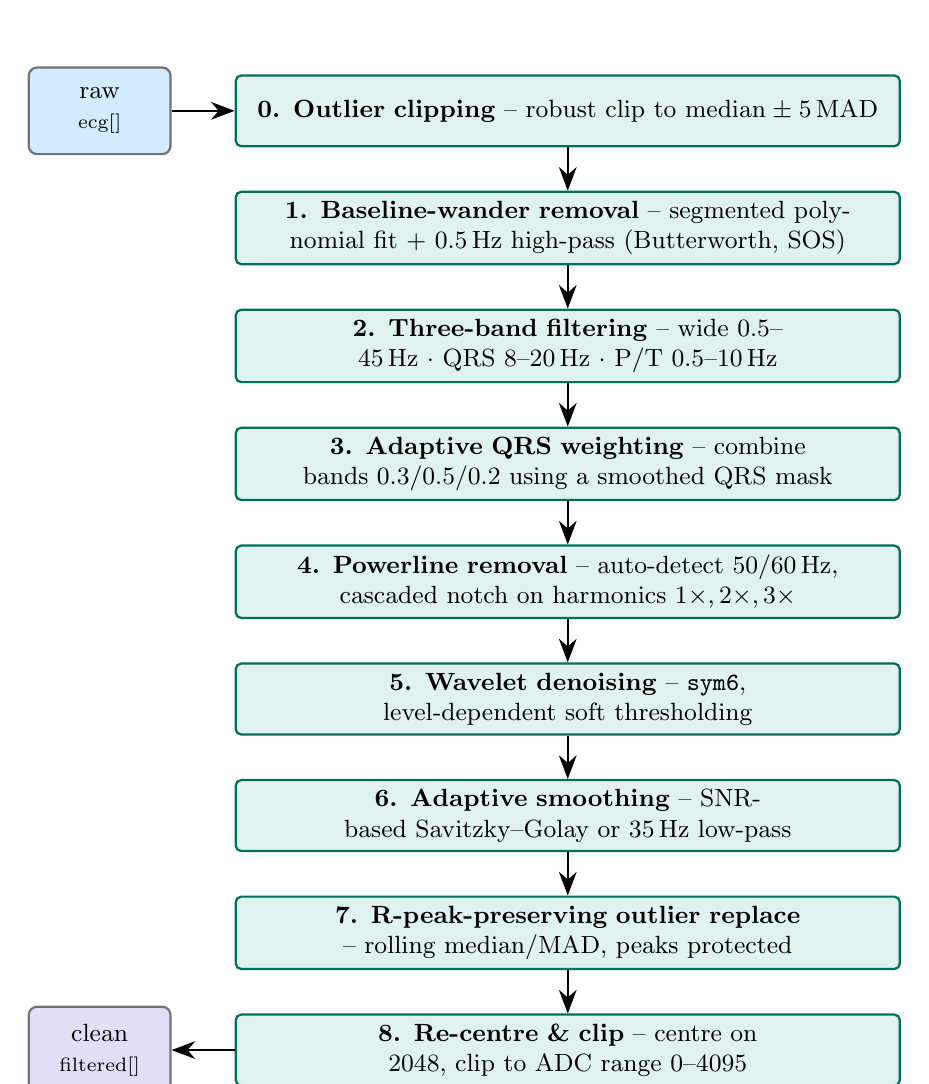
\begin{tikzpicture}[node distance=5.5mm]
    \node[stage] (s0) {\textbf{0. Outlier clipping} -- robust clip to
        $\text{median} \pm 5\,\text{MAD}$};
    \node[stage, below=of s0] (s1) {\textbf{1. Baseline-wander removal} --
        segmented polynomial fit + 0.5\,Hz high-pass (Butterworth, SOS)};
    \node[stage, below=of s1] (s2) {\textbf{2. Three-band filtering} --
        wide 0.5--45\,Hz $\cdot$ QRS 8--20\,Hz $\cdot$ P/T 0.5--10\,Hz};
    \node[stage, below=of s2] (s3) {\textbf{3. Adaptive QRS weighting} --
        combine bands $0.3 / 0.5 / 0.2$ using a smoothed QRS mask};
    \node[stage, below=of s3] (s4) {\textbf{4. Powerline removal} --
        auto-detect 50/60\,Hz, cascaded notch on harmonics $1\times,2\times,3\times$};
    \node[stage, below=of s4] (s5) {\textbf{5. Wavelet denoising} --
        \texttt{sym6}, level-dependent soft thresholding};
    \node[stage, below=of s5] (s6) {\textbf{6. Adaptive smoothing} --
        SNR-based Savitzky--Golay or 35\,Hz low-pass};
    \node[stage, below=of s6] (s7) {\textbf{7. R-peak-preserving outlier replace}
        -- rolling median/MAD, peaks protected};
    \node[stage, below=of s7] (s8) {\textbf{8. Re-centre \& clip} --
        centre on 2048, clip to ADC range 0--4095};

    \foreach \a/\b in {s0/s1,s1/s2,s2/s3,s3/s4,s4/s5,s5/s6,s6/s7,s7/s8}
        \draw[flow] (\a) -- (\b);

    \node[hw, left=8mm of s0, minimum width=18mm] (in) {raw\\\scriptsize ecg[]};
    \node[fe, left=8mm of s8, minimum width=18mm] (out) {clean\\\scriptsize filtered[]};
    \draw[flow] (in) -- (s0);
    \draw[flow] (s8) -- (out);
  \end{tikzpicture}
  \caption{The eight-stage \texttt{filter\_ecg\_signal()} pipeline. Each batch of
  raw samples flows top-to-bottom and emerges as a cleaned, ADC-scaled array.}
  \label{fig:dsp}
\end{figure}

\subsection*{Stage details}
\begin{description}[leftmargin=0pt,style=nextline]
  \item[0. Robust outlier clipping] Values are clipped to
        $\text{median} \pm 5\sigma$, where $\sigma$ is estimated from the median
        absolute deviation (MAD, scaled by $1.4826$). This removes gross spikes
        without being skewed by them, unlike a mean/standard-deviation clip.
  \item[1. Baseline-wander removal] For batches longer than five seconds the
        signal is detrended with a piecewise (segmented) polynomial fit to track
        non-stationary drift; then a 0.5\,Hz Butterworth high-pass
        (second-order-sections, zero-phase \texttt{sosfiltfilt}) removes the
        remainder.
  \item[2. Three-band filtering] The signal is split into three Butterworth
        band-passes tuned to different ECG features: a \emph{wide} band
        (0.5--45\,Hz) preserving overall morphology, a \emph{QRS} band (8--20\,Hz)
        isolating the sharp ventricular spike, and a \emph{P/T} band (0.5--10\,Hz)
        capturing the slower atrial and repolarisation waves.
  \item[3. Adaptive QRS weighting] A QRS energy mask is built with a sliding
        adaptive threshold ($\text{mean} + 1.8\,\text{std}$ over 1.5\,s windows)
        and smoothed. The three bands are recombined as
        $0.3\cdot\text{wide} + 0.5\cdot\text{QRS}\!\cdot\!\text{mask}
        + 0.2\cdot\text{P/T}\!\cdot\!(1-\text{mask})$, so the QRS band dominates
        during beats and the gentler bands dominate between them.
  \item[4. Powerline removal] If the mains frequency is not given, it is
        auto-detected via Welch power-spectral-density peaks near 50 or 60\,Hz.
        Cascaded \texttt{iirnotch} filters (two Q-factors, 35 and 50) then notch
        out the fundamental and its 2nd and 3rd harmonics.
  \item[5. Wavelet denoising] A \texttt{sym6} (Symlet-6) wavelet decomposition with
        level-dependent soft thresholding suppresses broadband noise while
        preserving ECG morphology; low-frequency detail is thresholded gently and
        high-frequency detail more aggressively.
  \item[6. Adaptive smoothing] The signal-to-noise ratio is estimated; very noisy
        batches get a short ($\approx$40\,ms) Savitzky--Golay smooth, moderately
        noisy batches a 35\,Hz low-pass, and clean batches are left untouched.
  \item[7. R-peak-preserving outlier replacement] R-peaks are located with the QRS
        band and an adaptive height threshold. A rolling median/MAD test then
        replaces residual outliers, but explicitly \emph{protects} the detected
        R-peak regions so the diagnostically important spikes are not flattened.
  \item[8. Re-centre and clip] Finally the signal is centred on 2048 (the middle of
        the 12-bit ADC range) and clipped to integer codes $0$--$4095$, matching
        the dashboard's fixed $y$-axis.
\end{description}

\paragraph{Output contract.} The function always returns a list of integers in
$[0,4095]$. Short batches (fewer than 20 samples) are returned unchanged, and any
stage that fails (for example wavelet reconstruction on an awkward length) falls
back gracefully so a single bad batch never breaks the stream.

%==============================================================================
\section{Frontend: Live Dashboard}
%==============================================================================

The dashboard is a single self-contained page,
\texttt{ecg/templates/ecg.html}, served at the site root. It pulls Chart.js
4.4.1 from a CDN and draws the heart waveform on a dark background, refreshed in
real time as cleaned batches arrive over the WebSocket.

\subsection{Rolling buffer and chart}
The page keeps a fixed-length \emph{rolling buffer} of 1000 samples (about four
seconds of signal at 250\,Hz). Each incoming batch is appended to the right while
the oldest samples drop off the left, producing the familiar scrolling-trace
effect of a bedside monitor. The chart's $y$-axis is pinned to the ADC range
$0$--$4095$ so the waveform's scale is stable, and animation is disabled so
updates are instantaneous.

\begin{table}[h]
  \centering\small
  \begin{tabular}{@{}ll@{}}
    \toprule
    \textbf{Setting} & \textbf{Value} \\
    \midrule
    Charting library   & Chart.js 4.4.1 (CDN) \\
    Chart type         & line, no point markers, slight tension (0.2) \\
    Buffer size        & 1000 samples ($\approx$4\,s window) \\
    $y$-axis range     & 0--4095 (fixed, matches ADC) \\
    $x$-axis           & linear sample index, hidden \\
    Animation          & disabled (real-time redraw) \\
    Trace colour       & lime on near-black background \\
    \bottomrule
  \end{tabular}
  \caption{Dashboard chart configuration.}
  \label{tab:chart}
\end{table}

\subsection{Receiving data}
The page opens a WebSocket back to the same host it was served from, so no
hard-coded server address is needed in the browser. Each message is a
\texttt{\{"filtered":[...]\}} array; the handler shifts the buffer and redraws.

\begin{lstlisting}[style=js,caption={Dashboard WebSocket handler and buffer update (abridged).}]
const BUFFER_SIZE = 1000;
let ecgBuffer = Array(BUFFER_SIZE).fill(0);

const ws = new WebSocket("ws://" + window.location.host + "/ws/ecg/");

ws.onmessage = (event) => {
  const msg = JSON.parse(event.data);
  const incoming = msg.filtered || msg.ecg;          // cleaned samples
  if (Array.isArray(incoming)) {
    // drop oldest, append newest -> scrolling trace
    ecgBuffer = ecgBuffer.slice(incoming.length).concat(incoming);
    ecgChart.data.datasets[0].data = ecgBuffer;
    ecgChart.update();
  }
};
\end{lstlisting}

Because the dashboard subscribes to the very same \texttt{ecg\_group} the server
broadcasts to, opening the page in several browsers shows the same live trace in
all of them simultaneously -- this is what makes the monitor ``remote'': any
machine that can reach the server can watch the patient's ECG.

%==============================================================================
\section{End-to-End Data Flow}
%==============================================================================

This section ties the tiers together and follows a single batch of samples from
the patient's chest to the clinician's screen.

\subsection{The journey of one batch}
\begin{enumerate}[noitemsep]
  \item The AD8232 outputs an analog ECG voltage; the ESP32 samples it 250 times,
        4\,ms apart ($\approx$1\,s of signal).
  \item The ESP32 serialises the batch as \texttt{\{"ecg":[\,\ldots 250 ints\ldots]\}}
        and sends it over the WebSocket to \texttt{ws://<server>:8000/ws/ecg/}.
  \item \texttt{ECGConsumer.receive()} parses the batch and calls
        \texttt{filter\_ecg\_signal()} (the eight-stage DSP pipeline).
  \item The cleaned array is broadcast to \texttt{ecg\_group} via
        \texttt{group\_send}, which invokes \texttt{send\_ecg()} on every member
        socket.
  \item Each dashboard receives \texttt{\{"filtered":[\,\ldots\,]\}}, appends it to
        its rolling buffer, and redraws the Chart.js trace.
\end{enumerate}

\begin{figure}[h]
  \centering
  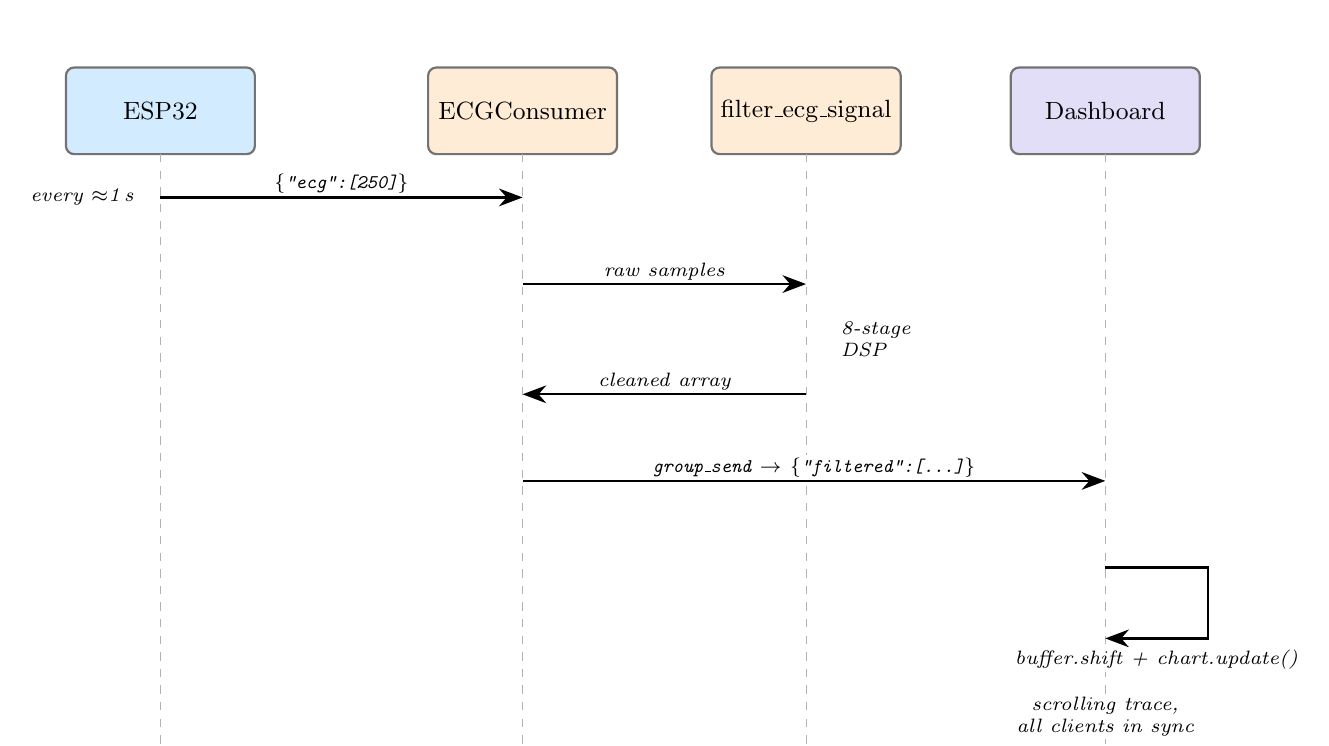
\begin{tikzpicture}[font=\small]
    % lifelines
    \def\esp{0}    \def\srv{4.6}  \def\dsp{8.2}  \def\web{12.0}
    \foreach \x/\name/\col in {\esp/ESP32/hwcol, \srv/ECGConsumer/bkcol,
                               \dsp/{filter\_ecg\_signal}/bkcol, \web/Dashboard/fecol}{
      \node[block, fill=\col, minimum width=24mm] (h\x) at (\x,0) {\name};
      \draw[dashed, gray!60] (\x,-0.55) -- (\x,-8.2);
    }

    % messages
    \draw[flow] (\esp,-1.1) -- (\srv,-1.1)
        node[midway,above,lbl]{\texttt{\{"ecg":[250]\}}};
    \node[lbl, anchor=east] at (\esp-0.3,-1.1) {every $\approx$1\,s};

    \draw[flow] (\srv,-2.2) -- (\dsp,-2.2)
        node[midway,above,lbl]{raw samples};
    \draw[flow] (\dsp,-3.6) -- (\srv,-3.6)
        node[midway,above,lbl]{cleaned array};
    \node[lbl, anchor=west, align=left] at (\dsp+0.4,-2.9) {8-stage\\DSP};

    \draw[flow] (\srv,-4.7) -- (\web,-4.7)
        node[midway,above,lbl]{\texttt{group\_send} $\rightarrow$ \texttt{\{"filtered":[...]\}}};

    % self-message at dashboard
    \draw[flow] (\web,-5.8) -- ++(1.3,0) -- ++(0,-0.9) -- ++(-1.3,0)
        node[midway,below=1mm,lbl,anchor=north]{buffer.shift + chart.update()};

    \node[lbl, anchor=north, align=center] at (\web,-7.4)
        {scrolling trace,\\all clients in sync};
  \end{tikzpicture}
  \caption{Sequence of one ECG batch: acquisition, filtering on the server, and
  fan-out to every connected dashboard. Both the device and the browsers share the
  single \texttt{ecg\_group}.}
  \label{fig:sequence}
\end{figure}

\subsection{Wire protocol}
Only two tiny JSON shapes cross the network, both on the same WebSocket path
\texttt{/ws/ecg/}:

\begin{table}[h]
  \centering\small
  \begin{tabular}{@{}lll@{}}
    \toprule
    \textbf{Direction} & \textbf{Shape} & \textbf{Payload} \\
    \midrule
    ESP32 $\rightarrow$ server   & \texttt{\{"ecg":[\,\ldots\,]\}}      & 250 raw ADC ints (0--4095) \\
    server $\rightarrow$ browser & \texttt{\{"filtered":[\,\ldots\,]\}} & 250 cleaned ADC ints (0--4095) \\
    \bottomrule
  \end{tabular}
  \caption{The two JSON message types. The dashboard also accepts an \texttt{ecg}
  key as a fallback.}
  \label{tab:protocol}
\end{table}

\subsection{Timing and throughput}
At 250\,Hz with 250-sample batches, the device emits roughly one message per
second, i.e.\ about 250 samples/s of sustained throughput per device. Filtering is
performed per batch, so end-to-end latency is dominated by the $\approx$1\,s it
takes to \emph{fill} a batch plus the (much smaller) DSP and network time. Reducing
\texttt{SAMPLE\_COUNT} would lower latency at the cost of more frequent, smaller
messages.

%==============================================================================
\section{Building \& Running the System}
%==============================================================================

This section walks through bringing the whole system up. You can run the dashboard
with real hardware or, for development, with the bundled software simulator.

\subsection{Prerequisites}
\begin{itemize}[noitemsep]
  \item Python 3.10+ on the server machine.
  \item Arduino IDE (or PlatformIO) with the ESP32 board support package, plus the
        \texttt{ArduinoWebsockets} and \texttt{ArduinoJson} libraries -- only needed
        for real hardware.
  \item An ESP32 development board and an AD8232 ECG module with electrodes -- only
        needed for real hardware.
\end{itemize}

\subsection{1. Backend server}
From the \texttt{holter\_monitor/} project directory:
\begin{lstlisting}[style=base,caption={Set up and run the Django/Channels server.}]
# create and activate a virtual environment
python -m venv venv
venv\Scripts\activate            # Windows
# source venv/bin/activate       # macOS / Linux

# install dependencies
pip install django channels daphne numpy scipy PyWavelets websockets

# apply Django's built-in migrations and start the server
python manage.py migrate
python manage.py runserver 0.0.0.0:8000
\end{lstlisting}

Because \texttt{daphne} and \texttt{channels} are installed and
\texttt{ASGI\_APPLICATION} is set, \texttt{runserver} starts the ASGI/WebSocket
server automatically. Binding to \texttt{0.0.0.0} makes the server reachable from
the ESP32 and from other machines on the LAN. Then open
\texttt{http://localhost:8000/} (or \texttt{http://<server-ip>:8000/} from another
device) to load the dashboard.

\subsection{2a. Run with the ESP32 (real ECG)}
\begin{enumerate}[noitemsep]
  \item Open \texttt{arduino/websocket\_ecg\_send\_data/websocket\_ecg\_send\_data.ino}.
  \item Set \texttt{ssid}, \texttt{password} and \texttt{websocket\_server\_host}
        (your server's LAN IP) near the top of the sketch.
  \item Wire the AD8232 output to \texttt{GPIO36} and power the board from 3.3\,V.
  \item Select your ESP32 board and port, then upload.
  \item Open the Serial Monitor at 115200 baud to watch it connect and stream;
        the dashboard trace should begin scrolling.
\end{enumerate}

\subsection{2b. Run without hardware (simulator)}
The repository includes \texttt{holter\_monitor/send\_fake\_data.py}, which connects
to the same WebSocket endpoint and pushes a synthetic ECG-like waveform (a noisy
sine) at the same rate the device would. With the server running:
\begin{lstlisting}[style=base,numbers=none]
python send_fake_data.py
\end{lstlisting}
This is the quickest way to verify the backend, DSP pipeline and dashboard without
any electronics. Note that the simulator feeds the \emph{same} \texttt{ecg\_group},
so the filtered output appears on every open dashboard exactly as real data would.

\subsection{Verifying it works}
\begin{itemize}[noitemsep]
  \item The dashboard page shows a scrolling lime waveform.
  \item The server console logs each received batch and broadcast.
  \item The browser console logs ``WebSocket connected'' and per-batch previews.
  \item With a real AD8232, the QRS spikes of the heartbeat are visible in the
        trace.
\end{itemize}

%==============================================================================
\section{Limitations \& Future Work}
\label{sec:limitations}
%==============================================================================

The project is a working proof of concept that demonstrates the full
acquisition\,$\rightarrow$\,processing\,$\rightarrow$\,visualisation loop. The
following items would be needed to harden it toward clinical or production use.

\subsection{Security}
\begin{itemize}[noitemsep]
  \item \textbf{Hard-coded credentials.} The firmware embeds the Wi-Fi SSID and
        password, and the server IP, as source constants. These should be moved to
        an un-committed secrets header (or provisioned at runtime) and never shared
        in a public repository.
  \item \textbf{Development Django settings.} \texttt{DEBUG = True},
        \texttt{ALLOWED\_HOSTS = ['*']} and a committed \texttt{SECRET\_KEY} are all
        unsafe for deployment. Set \texttt{DEBUG = False}, restrict the allowed
        hosts, and load the secret key from the environment.
  \item \textbf{No authentication or transport encryption.} The dashboard and the
        WebSocket are open to anyone on the network, and traffic is plain
        \texttt{ws://}. Patient ECG is sensitive data; production should add login,
        per-patient authorisation, and TLS (\texttt{wss://}/HTTPS).
\end{itemize}

\subsection{Scalability and robustness}
\begin{itemize}[noitemsep]
  \item \textbf{In-memory channel layer.} \texttt{InMemoryChannelLayer} works only
        within a single process. To run multiple workers or hosts, switch to
        \texttt{channels\_redis} with a Redis backend.
  \item \textbf{Single shared group.} All devices and viewers share one
        \texttt{ecg\_group}, so a second patient's device would mix into the same
        stream. Per-patient groups/rooms (e.g.\ \texttt{ecg\_<patient\_id>}) are
        needed for multiple simultaneous patients.
  \item \textbf{Latency.} Filling a 250-sample batch adds about one second of
        latency before display. Smaller batches reduce latency at the cost of more
        messages.
\end{itemize}

\subsection{Data and clinical features}
\begin{itemize}[noitemsep]
  \item \textbf{No persistence.} Samples are streamed but never stored;
        \texttt{ecg/models.py} is empty. Adding models for patients and recorded
        sessions would enable playback, export and offline review -- the defining
        feature of a true Holter monitor.
  \item \textbf{No analytics.} Heart-rate, R-R interval and arrhythmia detection
        could be layered on top of the existing R-peak detection already present in
        the DSP pipeline (Stage~7).
  \item \textbf{Single lead.} The AD8232 provides one lead; multi-lead acquisition
        would broaden diagnostic value.
\end{itemize}

\subsection{Hardware}
\begin{itemize}[noitemsep]
  \item \textbf{Power management.} Battery life, charging and low-power sleep
        between batches are not yet addressed.
  \item \textbf{Enclosure.} The wearable case is documented conceptually; published
        CAD/STL files and printed-part drawings would make the build reproducible.
\end{itemize}

\bigskip
\noindent\emph{In short: the signal path is complete and the DSP is genuinely
sophisticated; the remaining work is mostly the productionisation around it ---
security, persistence, multi-patient support and deployment.}


%------------------------------------------------------------------ references
\clearpage
\nocite{*}
\bibliographystyle{plain}
\bibliography{references}
\addcontentsline{toc}{section}{References}

\end{document}
